\documentclass{article}
\usepackage{amsmath}
\usepackage{fullpage}
\usepackage{multicol}
%\usepackage{graphicx}
\usepackage{tikz}
\usetikzlibrary{calc}
% \usepackage{pgfmath}
\usepackage[aux]{rerunfilecheck}

% Macros for MATH 110 course dates

\newcommand{\commonTheme}{metropolis}
\newcommand{\commonColorTheme}{metropolis}

\newcommand{\commonAuthor}{Edward Doolittle}
\newcommand{\commonInstitute}{Department of Indigenous Knowledge and
  Science \\ First Nations University of Canada}
\newcommand{\commonCourse}{MATH 110 Calculus I}
\newcommand{\commonTerm}{202510}
\newcommand{\commonDate}{January 6, 2025}

% Review Material

% Lab 0
\newcommand{\commonEventNegativeOne}{LabNegativeOne}
\newcommand{\commonDateLabNegativeOne}{Monday, January 6, 2025}
\newcommand{\commonTitleLabNegativeOne}{MATH 110 Lab 0}
\newcommand{\commonSubtitleLabNegativeOne}{No Lab; Course Opens}

% Section 001
\newcommand{\commonEventZeroZeroOne}{ZeroZeroOne}
\newcommand{\commonDateZeroZeroOne}{Tuesday, January 7, 2025}
\newcommand{\commonTitleZeroZeroOne}{MATH 110 Review 0.1}
\newcommand{\commonSubtitleZeroZeroOne}{Review of Algebra}
\newcommand{\commonPSTitleZeroZeroOne}{MATH 110 Review Problem Set 0.1}

% Section 00A
\newcommand{\commonEventZeroZeroA}{ZeroZeroA}
\newcommand{\commonDateZeroZeroA}{Tuesday, January 7, 2025}
\newcommand{\commonTitleZeroZeroA}{MATH 110 Review 0.A}
\newcommand{\commonSubtitleZeroZeroA}{Review of Inequalities and
  Absolute Values}
\newcommand{\commonPSTitleZeroZeroA}{MATH 110 Review Problem Set 0.A}

% Section 00B
\newcommand{\commonEventZeroZeroB}{ZeroZeroB}
\newcommand{\commonDateZeroZeroB}{Tuesday, January 7, 2025}
\newcommand{\commonTitleZeroZeroB}{MATH 110 Review 0.B}
\newcommand{\commonSubtitleZeroZeroB}{Review of Coordinate Geometry
  and Lines}
\newcommand{\commonPSTitleZeroZeroB}{MATH 110 Review Problem Set 0.B}

% Section 00C
\newcommand{\commonEventZeroZeroC}{ZeroZeroC}
\newcommand{\commonDateZeroZeroC}{Thursday, January 9, 2025}
\newcommand{\commonTitleZeroZeroC}{MATH 110 Review 0.C}
\newcommand{\commonSubtitleZeroZeroC}{Review of Graphs of Second
  Degree Equations}
\newcommand{\commonPSTitleZeroZeroC}{MATH 110 Review Problem Set 0.C}

% Section 00D
\newcommand{\commonEventZeroZeroD}{ZeroZeroD}
\newcommand{\commonDateZeroZeroD}{Thursday, January 9, 2025}
\newcommand{\commonTitleZeroZeroD}{MATH 110 Review 0.D}
\newcommand{\commonSubtitleZeroZeroD}{Review of Trigonometry}
\newcommand{\commonPSTitleZeroZeroD}{MATH 110 Review Problem Set 0.D}

% Section 011
\newcommand{\commonEventZeroOneOne}{ZeroOneOne}
\newcommand{\commonDateZeroOneOne}{Thursday, January 9, 2025}
\newcommand{\commonTitleZeroOneOne}{MATH 110 Review 1.1}
\newcommand{\commonSubtitleZeroOneOne}{Review of Functions}
\newcommand{\commonPSTitleZeroOneOne}{MATH 110 Review Problem Set 1.1}


% Main Course

% Lab 1
\newcommand{\commonEventZero}{LabZero}
\newcommand{\commonDateLabZero}{Monday, January 13, 2025}
\newcommand{\commonTitleLabZero}{MATH 110 Lab 1}
\newcommand{\commonSubtitleLabZero}{Quiz 0: STACK, Onboarding}

% Section 1.4
\newcommand{\commonEventOne}{ZeroOneFour}
\newcommand{\commonDateZeroOneFour}{Tuesday, January 14, 2025}
\newcommand{\commonTitleZeroOneFour}{MATH 110 Lecture 1.4}
\newcommand{\commonSubtitleZeroOneFour}{The Tangent and Velocity Problems}
\newcommand{\commonPSTitleZeroOneFour}{MATH 110 Problem Set 1.4}

% Section 1.5
\newcommand{\commonEventTwo}{ZeroOneFive}
\newcommand{\commonDateZeroOneFive}{Thursday, January 16, 2025}
\newcommand{\commonTitleZeroOneFive}{MATH 110 Lecture 1.5}
\newcommand{\commonSubtitleZeroOneFive}{The Limit of a Function}
\newcommand{\commonPSTitleZeroOneFive}{MATH 110 Problem Set 1.5}

% Lab 2
\newcommand{\commonEventThree}{LabOne}
\newcommand{\commonDateLabOne}{Monday, January 20, 2025}
\newcommand{\commonTitleLabOne}{MATH 110 Lab 2}
\newcommand{\commonSubtitleLabOne}{Quiz 1: Review}

% Section 1.6
\newcommand{\commonEventFour}{ZeroOneSix}
\newcommand{\commonDateZeroOneSix}{Tuesday, January 21, 2025}
\newcommand{\commonTitleZeroOneSix}{MATH 110 Lecture 1.6}
\newcommand{\commonSubtitleZeroOneSix}{Calculating Limits Using the Limit Laws}
\newcommand{\commonPSTitleZeroOneSix}{MATH 110 Problem Set 1.6}

% Section 1.7
\newcommand{\commonEventFive}{ZeroOneSeven}
\newcommand{\commonDateZeroOneSeven}{(Not covered)}
\newcommand{\commonTitleZeroOneSeven}{MATH 110 Lecture 1.7}
\newcommand{\commonSubtitleZeroOneSeven}{The Precise Definition of a Limit}
\newcommand{\commonPSTitleZeroOneSeven}{MATH 110 Problem Set 1.7}

% Section 1.8
\newcommand{\commonEventSix}{ZeroOneEight}
\newcommand{\commonDateZeroOneEight}{Thursday, January 23, 2025}
\newcommand{\commonTitleZeroOneEight}{MATH 110 Lecture 1.8}
\newcommand{\commonSubtitleZeroOneEight}{Continuity}
\newcommand{\commonPSTitleZeroOneEight}{MATH 110 Problem Set 1.8}

% Lab 3
\newcommand{\commonEventSeven}{LabTwo}
\newcommand{\commonDateLabTwo}{Monday, January 27, 2025}
\newcommand{\commonTitleLabTwo}{MATH 110 Lab 3}
\newcommand{\commonSubtitleLabTwo}{Quiz 2: Sections 1.4, 1.5}

% Section 2.1
\newcommand{\commonEventEight}{ZeroTwoOne}
\newcommand{\commonDateZeroTwoOne}{Tuesday, January 28, 2025}
\newcommand{\commonTitleZeroTwoOne}{MATH 110 Lecture 2.1}
\newcommand{\commonSubtitleZeroTwoOne}{Derivatives and Rates of Change}
\newcommand{\commonPSTitleZeroTwoOne}{MATH 110 Problem Set 2.1}

% Section 2.2
\newcommand{\commonEventNine}{ZeroTwoTwo}
\newcommand{\commonDateZeroTwoTwo}{Thursday, January 30, 2025}
\newcommand{\commonTitleZeroTwoTwo}{MATH 110 Lecture 2.2}
\newcommand{\commonSubtitleZeroTwoTwo}{The Derivative as a Function}
\newcommand{\commonPSTitleZeroTwoTwo}{MATH 110 Problem Set 2.2}

% Lab 4
\newcommand{\commonEventTen}{LabThree}
\newcommand{\commonDateMTOne}{Monday, February 3, 2025} 
\newcommand{\commonDateLabThree}{Monday, February 3, 2025}
\newcommand{\commonTitleLabThree}{MATH 110 Lab 4}
\newcommand{\commonSubtitleLabThree}{Midterm: Review, Chapter 1}

% Section 2.3
\newcommand{\commonEventEleven}{ZeroTwoThree}
\newcommand{\commonDateZeroTwoThree}{Tuesday, February 4, 2025}
\newcommand{\commonTitleZeroTwoThree}{MATH 110 Lecture 2.3}
\newcommand{\commonSubtitleZeroTwoThree}{Differentiation Formulas}
\newcommand{\commonPSTitleZeroTwoThree}{MATH 110 Problem Set 2.3}

% Section 2.4
\newcommand{\commonEventTwelve}{ZeroTwoFour}
\newcommand{\commonDateZeroTwoFour}{Thursday, February 6, 2025}
\newcommand{\commonTitleZeroTwoFour}{MATH 110 Lecture 2.4}
\newcommand{\commonSubtitleZeroTwoFour}{Derivatives of Trigonometric Functions}
\newcommand{\commonPSTitleZeroTwoFour}{MATH 110 Problem Set 2.4}

% Lab 5
\newcommand{\commonEventThirteen}{LabFour}
\newcommand{\commonDateLabFour}{Monday, February 10, 2025}
\newcommand{\commonTitleLabFour}{MATH 110 Lab 5}
\newcommand{\commonSubtitleLabFour}{Quiz 3: Sections 2.1, 2.2}

% Section 2.5
\newcommand{\commonEventFourteen}{ZeroTwoFive}
\newcommand{\commonDateZeroTwoFive}{Tuesday, February 11, 2025}
\newcommand{\commonTitleZeroTwoFive}{MATH 110 Lecture 2.5}
\newcommand{\commonSubtitleZeroTwoFive}{The Chain Rule}
\newcommand{\commonPSTitleZeroTwoFive}{MATH 110 Problem Set 2.5}

% Section 2.6
\newcommand{\commonEventFifteen}{ZeroTwoSix}
\newcommand{\commonDateZeroTwoSix}{Thursday, February 13, 2025}
\newcommand{\commonTitleZeroTwoSix}{MATH 110 Lecture 2.6}
\newcommand{\commonSubtitleZeroTwoSix}{Implicit Differentiation}
\newcommand{\commonPSTitleZeroTwoSix}{MATH 110 Problem Set 2.6}

% Lab 6
\newcommand{\commonEventSixteen}{LabFive}
\newcommand{\commonDateLabFive}{Monday, February 24, 2025}
\newcommand{\commonTitleLabFive}{MATH 110 Lab 6}
\newcommand{\commonSubtitleLabFive}{Quiz 4: Sections 2.3, 2.4}

% Section 2.7
\newcommand{\commonEventSeventeen}{ZeroTwoSeven}
\newcommand{\commonDateZeroTwoSeven}{Tuesday, February 25, 2025}
\newcommand{\commonTitleZeroTwoSeven}{MATH 110 Lecture 2.7}
\newcommand{\commonSubtitleZeroTwoSeven}{Rates of Change in the
  Natural and Social Sciences}
\newcommand{\commonPSTitleZeroTwoSeven}{MATH 110 Problem Set 2.7}

% Section 2.8
\newcommand{\commonEventEighteen}{ZeroTwoEight}
\newcommand{\commonDateZeroTwoEight}{Thursday, February 27, 2025}
\newcommand{\commonTitleZeroTwoEight}{MATH 110 Lecture 2.8}
\newcommand{\commonSubtitleZeroTwoEight}{Related Rates}
\newcommand{\commonPSTitleZeroTwoEight}{MATH 110 Problem Set 2.8}

% Lab 7
\newcommand{\commonEventNineteen}{LabSix}
\newcommand{\commonDateLabSix}{Monday, March 3, 2025}
\newcommand{\commonTitleLabSix}{MATH 110 Lab 7}
\newcommand{\commonSubtitleLabSix}{Quiz 5: Sections 2.5, 2.6}

% Section 3.1
\newcommand{\commonEventTwenty}{ZeroThreeOne}
\newcommand{\commonDateZeroThreeOne}{Tuesday, March 4, 2025}
\newcommand{\commonTitleZeroThreeOne}{MATH 110 Lecture 3.1}
\newcommand{\commonSubtitleZeroThreeOne}{Maximum and Minimum Values}
\newcommand{\commonPSTitleZeroThreeOne}{MATH 11 Problem Set 3.1}

% Section 3.2
\newcommand{\commonEventTwentyOne}{ZeroThreeTwo}
\newcommand{\commonDateZeroThreeTwo}{Thursday, March 6, 2025}
\newcommand{\commonTitleZeroThreeTwo}{MATH 110 Lecture 3.2}
\newcommand{\commonSubtitleZeroThreeTwo}{The Mean Value Theorem}
\newcommand{\commonPSTitleZeroThreeTwo}{MATH 110 Problem Set 3.2}

% Lab 8
\newcommand{\commonEventTwentyTwo}{LabSeven}
\newcommand{\commonDateMTTwo}{Monday, March 10, 2025}
\newcommand{\commonDateLabSeven}{Monday, March 10, 2025}
\newcommand{\commonTitleLabSeven}{MATH 110 Lab 8}
\newcommand{\commonSubtitleLabSeven}{Midterm: Chapter 2}

% Section 3.3
\newcommand{\commonEventTwentyThree}{ZeroThreeThree}
\newcommand{\commonDateZeroThreeThree}{Tuesday, March 11, 2025}
\newcommand{\commonTitleZeroThreeThree}{MATH 110 Lecture 3.3}
\newcommand{\commonSubtitleZeroThreeThree}{How Derivatives Affect the
  Shape of a Graph}
\newcommand{\commonPSTitleZeroThreeThree}{MATH 110 Problem Set 3.3}

% Section 3.4
\newcommand{\commonEventTwentyFour}{ZeroThreeFour}
\newcommand{\commonDateZeroThreeFour}{Thursday, March 13, 2025}
\newcommand{\commonTitleZeroThreeFour}{MATH 110 Lecture 3.4}
\newcommand{\commonSubtitleZeroThreeFour}{Limits at Infinity;
  Horizontal Asymptotes}
\newcommand{\commonPSTitleZeroThreeFour}{MATH 110 Problem Set 3.4}

% Lab 9
\newcommand{\commonEventTwentyFive}{LabEight}
\newcommand{\commonDateLabEight}{Monday, March 17, 2025}
\newcommand{\commonTitleLabEight}{MATH 110 Lab 9}
\newcommand{\commonSubtitleLabEight}{Quiz 6: Sections 3.1, 3.2}

% Section 3.5
\newcommand{\commonEventTwentySix}{ZeroThreeFive}
\newcommand{\commonDateZeroThreeFive}{Tuesday, March 18, 2025}
\newcommand{\commonTitleZeroThreeFive}{MATH 110 Lecture 3.5}
\newcommand{\commonSubtitleZeroThreeFive}{Summary of Curve Sketching}
\newcommand{\commonPSTitleZeroThreeFive}{MATH 110 Problem Set 3.5}

% Section 3.7
\newcommand{\commonEventTwentySeven}{ZeroThreeSeven}
\newcommand{\commonDateZeroThreeSeven}{Thursday, March 20, 2025}
\newcommand{\commonTitleZeroThreeSeven}{MATH 110 Lecture 3.7}
\newcommand{\commonSubtitleZeroThreeSeven}{Optimization Problems}
\newcommand{\commonPSTitleZeroThreeSeven}{MATH 110 Problem Set 3.7}

% Lab 10
\newcommand{\commonEventTwentyEight}{LabNine}
\newcommand{\commonDateLabNine}{Monday, March 24, 2025}
\newcommand{\commonTitleLabNine}{MATH 110 Lab 10}
\newcommand{\commonSubtitleLabNine}{Quiz 7: Sections 3.3, 3.4}

% Section 4.1
\newcommand{\commonEventTwentyNine}{ZeroFourOne}
\newcommand{\commonDateZeroFourOne}{Tuesday, March 25, 2025}
\newcommand{\commonTitleZeroFourOne}{MATH 110 Lecture 4.1}
\newcommand{\commonSubtitleZeroFourOne}{Areas and Distances}
\newcommand{\commonPSTitleZeroFourOne}{MATH 110 Problem Set 4.1}

% Section 4.2
\newcommand{\commonEventThirty}{ZeroFourTwo}
\newcommand{\commonDateZeroFourTwo}{Thursday, March 27, 2025}
\newcommand{\commonTitleZeroFourTwo}{MATH 110 Lecture 4.2}
\newcommand{\commonSubtitleZeroFourTwo}{The Definite Integral}
\newcommand{\commonPSTitleZeroFourTwo}{MATH 110 Problem Set 4.2}

% Lab 11
\newcommand{\commonEventThirtyOne}{LabTen}
\newcommand{\commonDateLabTen}{Monday, March 31, 2025}
\newcommand{\commonTitleLabTen}{MATH 110 Lab 11}
\newcommand{\commonSubtitleLabTen}{Quiz 8: Sections 3.5, 3.7}

% Section 4.3
\newcommand{\commonEventThirtyTwo}{ZeroFourThree}
\newcommand{\commonDateZeroFourThree}{Tuesday, April 1, 2025}
\newcommand{\commonTitleZeroFourThree}{MATH 110 Lecture 4.3}
\newcommand{\commonSubtitleZeroFourThree}{The Fundamental Theorem of Calculus}
\newcommand{\commonPSTitleZeroFourThree}{MATH 110 Problem Set 4.3}

% Section 4.4
\newcommand{\commonEventThirtyThree}{ZeroFourFour}
\newcommand{\commonDateZeroFourFour}{Thursday, April 3, 2025}
\newcommand{\commonTitleZeroFourFour}{MATH 110 Lecture 4.4}
\newcommand{\commonSubtitleZeroFourFour}{Indefinite Integrals and the
  Net Change Theorem}
\newcommand{\commonPSTitleZeroFourFour}{MATH 110 Problem Set 4.4}

% Lab 12
\newcommand{\commonEventThirtyFour}{LabEleven}
\newcommand{\commonDateLabEleven}{Monday, April 7, 2025}
\newcommand{\commonTitleLabEleven}{MATH 110 Lab 12}
\newcommand{\commonSubtitleLabEleven}{Quiz 9: Sections 4.1, 4.2}

% Section 4.5
\newcommand{\commonEventThirtyFive}{ZeroFourFive}
\newcommand{\commonDateZeroFourFive}{Tuesday, April 8, 2025}
\newcommand{\commonTitleZeroFourFive}{MATH 110 Lecture 4.5}
\newcommand{\commonSubtitleZeroFourFive}{The Substitution Rule}
\newcommand{\commonPSTitleZeroFourFive}{MATH 110 Problem Set 4.5}

% Section 5.1
\newcommand{\commonEventThirtySix}{ZeroFiveOne}
\newcommand{\commonDateZeroFiveOne}{Thursday, April 10, 2025}
\newcommand{\commonTitleZeroFiveOne}{MATH 110 Lecture 5.1}
\newcommand{\commonSubtitleZeroFiveOne}{Areas Between Curves}
\newcommand{\commonPSTitleZeroFiveOne}{MATH 110 Problem Set 5.1}

% Lab 13
\newcommand{\commonEventThirtySeven}{LabTwelve}
\newcommand{\commonDateLabTwelve}{Monday, April 14, 2025}
\newcommand{\commonTitleLabTwelve}{MATH 110 Review Lab}
\newcommand{\commonSubtitleLabTwelve}{Bonus Quiz 10: Sections 4.3, 4.4}

% Final Class
\newcommand{\commonEventThirtyEight}{FinalClass}
\newcommand{\commonDateFinalClass}{Tuesday, April 15, 2025}
\newcommand{\commonTitleFinalClass}{MATH 110 Review Class}
\newcommand{\commonSubtitleFinalClass}{Answer Questions, Review for Exam}

% Final Exam
\newcommand{\commonEventThirtyNine}{Final}
\newcommand{\commonDateFinal}{Thursday, April 22, 2025}
\newcommand{\commonTitleFinal}{MATH 110 Final Exam}
\newcommand{\commonSubtitleFinal}{Comprehensive Exam: All Sections}

% Orphaned -- no longer part of the course

% Section 2.9
\newcommand{\commonDateZeroTwoNine}{Not part of the course}
\newcommand{\commonTitleZeroTwoNine}{MATH 110 Lecture 2.9}
\newcommand{\commonSubtitleZeroTwoNine}{Linear Approximations and Differentials}
\newcommand{\commonPSTitleZeroTwoNine}{MATH 110 Problem Set 2.9}


% % Introduction
% \newcommand{\commonEventOneDate}{Wednesday, September 8, 2010}
% \newcommand{\commonEventOneDesc}{Introduction to the Course}
% \newcommand{\commonDateZeroZeroZero}{September 8, 2010}
% \newcommand{\commonTitleZeroZeroZero}{MATH 104 Introduction}
% \newcommand{\commonSubtitleZeroZeroZero}{Outline of the Course}

% % Lecture 1
% \newcommand{\commonEventTwoDate}{Friday, September 10, 2010}
% \newcommand{\commonEventTwoDesc}{Lecture 1: Algebra}
% \newcommand{\commonDateZeroZeroOne}{September 10, 2010}
% \newcommand{\commonTitleZeroZeroOne}{MATH 104 Lecture 1}
% \newcommand{\commonSubtitleZeroZeroOne}{Review of Algebra}
% % associated evaluation ... factor this out?
% \newcommand{\commonPSTitleZeroZeroOne}{MATH 104 Problem Set 1}
% \newcommand{\commonEvalZeroZeroOne}{Quiz 1}
% \newcommand{\commonEvalDateZeroZeroOne}{Wednesday, September 15, 2010}

% % Lecture 2
% \newcommand{\commonEventThreeDate}{Monday, September 13, 2010}
% \newcommand{\commonEventThreeDesc}{Lecture 2: Appendix A}
% \newcommand{\commonDateZeroZeroA}{September 13, 2010}
% \newcommand{\commonTitleZeroZeroA}{MATH 104 Lecture 2}
% \newcommand{\commonSubtitleZeroZeroA}{Appendix A: Numbers, Inequalities, 
%   and Absolute Values}
% % associated evaluation ... factor this out?
% \newcommand{\commonPSTitleZeroZeroA}{MATH 104 Problem Set 2}
% \newcommand{\commonEvalZeroZeroA}{Quiz 2}
% \newcommand{\commonEvalDateZeroZeroA}{Wednesday, September 22, 2010}

% % Review 1
% \newcommand{\commonEventFourDate}{Wednesday, September 15, 2010}
% \newcommand{\commonEventFourDesc}{Review 1: Review Algebra; Quiz 1; Review Appendix A}
% \newcommand{\commonDateRZeroOne}{September 15, 2010}
% \newcommand{\commonTitleRZeroOne}{MATH 104 Review 1}
% \newcommand{\commonSubtitleRZeroOne}{Review of Algebra, Appendix A}

% % Lecture 3
% \newcommand{\commonEventFiveDate}{Friday, September 17, 2010}
% \newcommand{\commonEventFiveDesc}{Lecture 3: Appendix B}
% \newcommand{\commonDateZeroZeroB}{September 17, 2010}
% \newcommand{\commonTitleZeroZeroB}{MATH 104 Lecture 3}
% \newcommand{\commonSubtitleZeroZeroB}{Appendix B: Coordinate Geometry and Lines}
% % associated evaluation ... factor this out?
% \newcommand{\commonPSTitleZeroZeroB}{MATH 104 Problem Set 3}
% \newcommand{\commonEvalZeroZeroB}{Quiz 2}
% \newcommand{\commonEvalDateZeroZeroB}{Wednesday, September 22, 2010}

% % Lecture 4
% \newcommand{\commonEventSixDate}{Monday, Sepbember 20, 2010}
% \newcommand{\commonEventSixDesc}{Lecture 4: Appendix C}
% \newcommand{\commonDateZeroZeroC}{September 20, 2010}
% \newcommand{\commonTitleZeroZeroC}{MATH 104 Lecture 4}
% \newcommand{\commonSubtitleZeroZeroC}{Appendix C: Graphs of Second-Degree Equations}
% % associated evaluation ... factor this out?
% \newcommand{\commonPSTitleZeroZeroC}{MATH 104 Problem Set 4}
% \newcommand{\commonEvalZeroZeroC}{Midterm 0}
% \newcommand{\commonEvalDateZeroZeroC}{Wednesday, September 29, 2010}

% % Review 2
% \newcommand{\commonEventSevenDate}{Wednesday, September 22, 2010}
% \newcommand{\commonEventSevenDesc}{Review 2: Review Appendix B; Quiz 2; Review Appendix C}
% \newcommand{\commonDateRZeroTwo}{September 22, 2010}
% \newcommand{\commonTitleRZeroTwo}{MATH 104 Review 2}
% \newcommand{\commonSubtitleRZeroTwo}{Review of Appendices B and C}

% % Lecture 5
% \newcommand{\commonEventEightDate}{Friday, September 24, 2010}
% \newcommand{\commonEventEightDesc}{Lecture 5: Appendix D}
% \newcommand{\commonDateZeroZeroD}{September 24, 2010}
% \newcommand{\commonTitleZeroZeroD}{MATH 104 Lecture 5}
% \newcommand{\commonSubtitleZeroZeroD}{Appendix D: Trigonometry}
% % associated evaluation ... factor this out?
% \newcommand{\commonPSTitleZeroZeroD}{MATH 104 Problem Set 5}
% \newcommand{\commonEvalZeroZeroD}{Midterm 0}
% \newcommand{\commonEvalDateZeroZeroD}{Wednesday, September 29, 2010}

% % Lecture 6
% \newcommand{\commonEventNineDate}{Monday, September 27, 2010}
% \newcommand{\commonEventNineDesc}{Lecture 6: Section 1.1}
% \newcommand{\commonDateZeroOneOne}{September 27, 2010}
% \newcommand{\commonTitleZeroOneOne}{MATH 104 Lecture 6}
% \newcommand{\commonSubtitleZeroOneOne}{Section 1.1: Four Ways to Represent a Function}
% % associated evaluation ... factor this out?
% \newcommand{\commonPSTitleZeroOneOne}{MATH 104 Problem Set 6}
% \newcommand{\commonEvalZeroOneOne}{Quiz 3}
% \newcommand{\commonEvalDateZeroOneOne}{Wednesday, October 6, 2010}

% % Review 3
% \newcommand{\commonEventTenDate}{Wednesday, September 29, 2010}
% \newcommand{\commonEventTenDesc}{Review 3: Review Appendix D; 
%   Self-Assessment Midterm 0}
% \newcommand{\commonDateRZeroThree}{September 29, 2010}
% \newcommand{\commonTitleRZeroThree}{MATH 104 Review 3}
% \newcommand{\commonSubtitleRZeroThree}{Review of Appendix D}

% % Lecture 7
% \newcommand{\commonEventElevenDate}{Friday, October 1, 2010}
% \newcommand{\commonEventElevenDesc}{Lecture 7: Section 1.2}
% \newcommand{\commonDateZeroOneTwo}{October 1, 2010}
% \newcommand{\commonTitleZeroOneTwo}{MATH 104 Lecture 7}
% \newcommand{\commonSubtitleZeroOneTwo}{Section 1.2: Mathematical Models: A Catalog of Essential Functions}
% % associated evaluation ... factor this out?
% \newcommand{\commonPSTitleZeroOneTwo}{MATH 104 Problem Set 7}
% \newcommand{\commonEvalZeroOneTwo}{Quiz 3}
% \newcommand{\commonEvalDateZeroOneTwo}{Wednesday, October 6, 2010}

% % Lecture 8
% \newcommand{\commonEventTwelveDate}{Monday, October 4, 2010}
% \newcommand{\commonEventTwelveDesc}{Lecture 8: Section 1.3}
% \newcommand{\commonDateZeroOneThree}{October 4, 2010}
% \newcommand{\commonTitleZeroOneThree}{MATH 104 Lecture 8}
% \newcommand{\commonSubtitleZeroOneThree}{Section 1.3: New Functions from Old Functions}
% % associated evaluation ... factor this out?
% \newcommand{\commonPSTitleZeroOneThree}{MATH 104 Problem Set 8}
% \newcommand{\commonEvalZeroOneThree}{Quiz 4}
% \newcommand{\commonEvalDateZeroOneThree}{Wednesday, October 13, 2010}

% % Review 4
% \newcommand{\commonEventThirteenDate}{Wednesday, October 6, 2010}
% \newcommand{\commonEventThirteenDesc}{Review 4: Review 1.1, 1.2; Quiz 3}
% \newcommand{\commonDateROneOne}{October 6, 2010}
% \newcommand{\commonTitleROneOne}{MATH 104 Review 4}
% \newcommand{\commonSubtitleROneOne}{Reveiw of 1.1, 1.2}

% % Lecture 9
% \newcommand{\commonEventFourteenDate}{Friday, October 8, 2010}
% \newcommand{\commonEventFourteenDesc}{Lecture 9: Section 1.4}
% \newcommand{\commonDateZeroOneFour}{October 8, 2010}
% \newcommand{\commonTitleZeroOneFour}{MATH 104 Lecture 9}
% \newcommand{\commonSubtitleZeroOneFour}{Section 1.4: Graphing Calculators and Computers}
% % associated evaluation ... factor this out?
% \newcommand{\commonPSTitleZeroOneFour}{MATH 104 Problem Set 9}
% \newcommand{\commonEvalZeroOneFour}{Quiz 4}
% \newcommand{\commonEvalDateZeroOneFour}{Wednesday, October 13, 2010}

% % Thanksgiving holiday
% \newcommand{\commonEventFifteenDate}{Monday, October 11, 2010}
% \newcommand{\commonEventFifteenDesc}{No class: Thanksgiving holiday}

% % Review 5
% \newcommand{\commonEventSixteenDate}{Wednesday, October 13, 2010}
% \newcommand{\commonEventSixteenDesc}{Review 5: Review 1.3, 1.4; Quiz 4}
% \newcommand{\commonDateROneTwo}{October 13, 2010}
% \newcommand{\commonTitleROneTwo}{MATH 104 Review 5}
% \newcommand{\commonSubtitleOneRTwo}{Review of 1.3, 1.4}

% % Lecture 10
% \newcommand{\commonEventSeventeenDate}{Friday, October 15, 2010}
% \newcommand{\commonEventSeventeenDesc}{Lecture 10: Section 1.5}
% \newcommand{\commonDateZeroOneFive}{October 15, 2010}
% \newcommand{\commonTitleZeroOneFive}{MATH 104 Lecture 10}
% \newcommand{\commonSubtitleZeroOneFive}{Section 1.5: Exponential Functions}
% % associated evaluation ... factor this out?
% \newcommand{\commonPSTitleZeroOneFive}{MATH 104 Problem Set 10}
% \newcommand{\commonEvalZeroOneFive}{Quiz 5}
% \newcommand{\commonEvalDateZeroOneFive}{Wednesday, October 20, 2010}

% % Lecture 11
% \newcommand{\commonEventEighteenDate}{Monday, October 18, 2010}
% \newcommand{\commonEventEighteenDesc}{Lecture 11: Section 1.6}
% \newcommand{\commonDateZeroOneSix}{October 18, 2010}
% \newcommand{\commonTitleZeroOneSix}{MATH 104 Lecture 11}
% \newcommand{\commonSubtitleZeroOneSix}{Section 1.6: Inverse Functions and Logarithms}
% % associated evaluation ... factor this out?
% \newcommand{\commonPSTitleZeroOneSix}{MATH 104 Problem Set 11}
% \newcommand{\commonEvalZeroOneSix}{Midterm 1}
% \newcommand{\commonEvalDateZeroOneSix}{Wednesday, October 27, 2010}

% % Review 6
% \newcommand{\commonEventNineteenDate}{Wednesday, October 20, 2010}
% \newcommand{\commonEventNineteenDesc}{Review 6: Review 1.5; Quiz 5; Review 1.6}
% \newcommand{\commonDateROneThree}{October 20, 2010}
% \newcommand{\commonDateZeroOneR}{October 20, 2010}
% \newcommand{\commonTitleROneThree}{MATH 104 Review 6}
% \newcommand{\commonSubtitleROneThree}{Review of 1.5, 1.6}
% % associated evaluation ... factor this out?
% \newcommand{\commonPSTitleZeroOneR}{MATH 104 Problem Set R1}
% \newcommand{\commonEvalZeroOneR}{Midterm 1}
% \newcommand{\commonEvalDateZeroOneR}{Wednesday, October 27, 2010}

% % Lecture 12
% \newcommand{\commonEventTwentyDate}{Friday, October 22, 2010}
% \newcommand{\commonEventTwentyDesc}{Lecture 12: Section 2.1}
% \newcommand{\commonDateZeroTwoOne}{October 22, 2010}
% \newcommand{\commonTitleZeroTwoOne}{MATH 104 Lecture 12}
% \newcommand{\commonSubtitleZeroTwoOne}{Section 2.1: The Tangent and Velocity Problems}
% % associated evaluation ... factor this out?
% \newcommand{\commonPSTitleZeroTwoOne}{MATH 104 Problem Set 12}
% \newcommand{\commonEvalZeroTwoOne}{Quiz 6}
% \newcommand{\commonEvalDateZeroTwoOne}{Wednesday, November 3, 2010}

% % Lecture 13
% \newcommand{\commonEventTwentyOneDate}{Monday, October 25, 2010}
% \newcommand{\commonEventTwentyOneDesc}{Lecture 13: Section 2.2(a)}
% \newcommand{\commonDateZeroTwoTwoa}{October 25, 2010}
% \newcommand{\commonTitleZeroTwoTwoa}{MATH 104 Lecture 13}
% \newcommand{\commonSubtitleZeroTwoTwoa}{Section 2.2(a): The Limit of a Function I}
% % associated evaluation ... factor this out?
% \newcommand{\commonPSTitleZeroTwoTwoa}{MATH 104 Problem Set 13}
% \newcommand{\commonEvalZeroTwoTwoa}{Quiz 6}
% \newcommand{\commonEvalDateZeroTwoTwoa}{Wednesday, November 3, 2010}

% % Midterm Test 1
% % October 27, 2010
% \newcommand{\commonEventTwentyTwoDate}{Wednesday, October 27, 2010}
% \newcommand{\commonEventTwentyTwoDesc}{Midterm Test 1: Chapter 1}

% % Lecture 14
% \newcommand{\commonEventTwentyThreeDate}{Friday, October 29, 2010}
% \newcommand{\commonEventTwentyThreeDesc}{Lecture 14: Section 2.2(b)}
% \newcommand{\commonDateZeroTwoTwob}{October 29, 2010}
% \newcommand{\commonTitleZeroTwoTwob}{MATH 104 Lecture 14}
% \newcommand{\commonSubtitleZeroTwoTwob}{Section 2.2(b): The Limit of a Function II}
% % associated evaluation ... factor this out?
% \newcommand{\commonPSTitleZeroTwoTwob}{MATH 104 Problem Set 14}
% \newcommand{\commonEvalZeroTwoTwob}{Quiz 6}
% \newcommand{\commonEvalDateZeroTwoTwob}{Wednesday, November 3, 2010}

% % Lecture 15
% \newcommand{\commonEventTwentyFourDate}{Monday, November 1, 2010}
% \newcommand{\commonEventTwentyFourDesc}{Lecture 15: Section 2.3}
% \newcommand{\commonDateZeroTwoThree}{November 1, 2010}
% \newcommand{\commonTitleZeroTwoThree}{MATH 104 Lecture 15}
% \newcommand{\commonSubtitleZeroTwoThree}{Section 2.3: Calculating Limits Using the Limit Laws}
% % associated evaluation ... factor this out?
% \newcommand{\commonPSTitleZeroTwoThree}{MATH 104 Problem Set 15}
% \newcommand{\commonEvalZeroTwoThree}{Quiz 7}
% \newcommand{\commonEvalDateZeroTwoThree}{Wednesday, November 10, 2010}

% % Review 7
% \newcommand{\commonEventTwentyFiveDate}{Wednesday, November 3, 2010}
% \newcommand{\commonEventTwentyFiveDesc}{Review 7: Review 2.1, 2.2; Quiz 6; Review 2.3}
% \newcommand{\commonDateRTwoOne}{November 3, 2010}
% \newcommand{\commonTitleRTwoOne}{MATH 104 Review 7}
% \newcommand{\commonSubtitleRTwoOne}{Review of 2.1, 2.2, 2.3}

% % Lecture 16
% \newcommand{\commonEventTwentySixDate}{Friday, November 5, 2010}
% \newcommand{\commonEventTwentySixDesc}{Lecture 16: Section 2.5}
% \newcommand{\commonDateZeroTwoFive}{November 5, 2010}
% \newcommand{\commonTitleZeroTwoFive}{MATH 104 Lecture 16}
% \newcommand{\commonSubtitleZeroTwoFive}{Section 2.5: Continuity}
% % associated evaluation ... factor this out?
% \newcommand{\commonPSTitleZeroTwoFive}{MATH 104 Problem Set 16}
% \newcommand{\commonEvalZeroTwoFive}{Quiz 7}
% \newcommand{\commonEvalDateZeroTwoFive}{Wednesday, November 10, 2010}

% % Lecture 17
% \newcommand{\commonEventTwentySevenDate}{Monday, November 8, 2010}
% \newcommand{\commonEventTwentySevenDesc}{Lecture 17: Section 2.6}
% \newcommand{\commonDateZeroTwoSix}{November 8, 2010}
% \newcommand{\commonTitleZeroTwoSix}{MATH 104 Lecture 17}
% \newcommand{\commonSubtitleZeroTwoSix}{Section 2.6: Limits at Infinity: Horizontal Asymptotes}
% % associated evaluation ... factor this out?
% \newcommand{\commonPSTitleZeroTwoSix}{MATH 104 Problem Set 17}
% \newcommand{\commonEvalZeroTwoSix}{Quiz 8}
% \newcommand{\commonEvalDateZeroTwoSix}{Wednesday, November 17, 2010}

% % Review 8
% \newcommand{\commonEventTwentyEightDate}{Wednesday, November 10, 2010}
% \newcommand{\commonEventTwentyEightDesc}{Review 8: Review 2.5; Quiz 7; Review 2.6}
% \newcommand{\commonDateRTwoTwo}{November 10, 2010}
% \newcommand{\commonTitleRTwoTwo}{MATH 104 Review 8}
% \newcommand{\commonSubtitleRTwoTwo}{Review of 2.5, 2.6}

% % Lecture 18
% \newcommand{\commonEventTwentyNineDate}{Friday, November 12, 2010}
% \newcommand{\commonEventTwentyNineDesc}{Lecture 18: Section 2.7}
% \newcommand{\commonDateZeroTwoSeven}{November 12, 2010}
% \newcommand{\commonTitleZeroTwoSeven}{MATH 104 Lecture 18}
% \newcommand{\commonSubtitleZeroTwoSeven}{Section 2.7: Derivatives and Rates of Change}
% % associated evaluation ... factor this out?
% \newcommand{\commonPSTitleZeroTwoSeven}{MATH 104 Problem Set 18}
% \newcommand{\commonEvalZeroTwoSeven}{Quiz 8}
% \newcommand{\commonEvalDateZeroTwoSeven}{Wednesday, November 17, 2010}

% % Lecture 19
% \newcommand{\commonEventThirtyDate}{Monday, November 15, 2010}
% \newcommand{\commonEventThirtyDesc}{Lecture 19: Section 2.8}
% \newcommand{\commonDateZeroTwoEight}{November 15, 2010}
% \newcommand{\commonTitleZeroTwoEight}{MATH 104 Lecture 19}
% \newcommand{\commonSubtitleZeroTwoEight}{Section 2.8: The Derivative as a Function}
% % associated evaluation ... factor this out?
% \newcommand{\commonPSTitleZeroTwoEight}{MATH 104 Problem Set 19}
% \newcommand{\commonEvalZeroTwoEight}{Midterm 2}
% \newcommand{\commonEvalDateZeroTwoEight}{Wednesday, November 24, 2010}

% % Review 9
% % November 17, 2010
% \newcommand{\commonEventThirtyOneDate}{Wednesday, November 17, 2010}
% \newcommand{\commonEventThirtyOneDesc}{Review 9: Review 2.7; Quiz 8; Review 2.8}
% \newcommand{\commonDateRTwoThree}{November 17, 2010}
% \newcommand{\commonTitleRTwoThree}{MATH 104 Review 9}
% \newcommand{\commonSubtitleRTwoThree}{Review of 2.7, 2.8}

% % Lecture 20
% \newcommand{\commonEventThirtyTwoDate}{Friday, November 19, 2010}
% \newcommand{\commonEventThirtyTwoDesc}{Lecture 20: Section 3.1}
% \newcommand{\commonDateZeroThreeOne}{November 19, 2010}
% \newcommand{\commonTitleZeroThreeOne}{MATH 104 Lecture 20}
% \newcommand{\commonSubtitleZeroThreeOne}{Section 3.1: Derivatives of Polynomials and Exponential Functions}
% % associated evaluation ... factor this out?
% \newcommand{\commonPSTitleZeroThreeOne}{MATH 104 Problem Set 20}
% \newcommand{\commonEvalZeroThreeOne}{Quiz 9}
% \newcommand{\commonEvalDateZeroThreeOne}{Wednesday, December 1, 2010}

% % Lecture 21
% \newcommand{\commonEventThirtyThreeDate}{Monday, November 22, 2010}
% \newcommand{\commonEventThirtyThreeDesc}{Lecture 21: Section 3.2}
% \newcommand{\commonDateZeroThreeTwo}{November 22, 2010}
% \newcommand{\commonTitleZeroThreeTwo}{MATH 104 Lecture 21}
% \newcommand{\commonSubtitleZeroThreeTwo}{Section 3.2: The Product and Quotient Rules}
% % associated evaluation ... factor this out?
% \newcommand{\commonPSTitleZeroThreeTwo}{MATH 104 Problem Set 21}
% \newcommand{\commonEvalZeroThreeTwo}{Quiz 9}
% \newcommand{\commonEvalDateZeroThreeTwo}{Wednesday, December 1, 2010}

% % Midterm Test 2
% \newcommand{\commonEventThirtyFourDate}{Wednesday, November 24, 2010}
% \newcommand{\commonEventThirtyFourDesc}{Midterm Test 2: Chapter 2}

% % Lecture 22
% \newcommand{\commonEventThirtyFiveDate}{Friday, November 26, 2010}
% \newcommand{\commonEventThirtyFiveDesc}{Lecture 22: Section 3.3}
% \newcommand{\commonDateZeroThreeThree}{November 26, 2010}
% \newcommand{\commonTitleZeroThreeThree}{MATH 104 Lecture 22}
% \newcommand{\commonSubtitleZeroThreeThree}{Section 3.3: Derivatives of Trigonometric Functions}
% % associated evaluation ... factor this out?
% \newcommand{\commonPSTitleZeroThreeThree}{MATH 104 Problem Set 22}
% \newcommand{\commonEvalZeroThreeThree}{Quiz 9}
% \newcommand{\commonEvalDateZeroThreeThree}{Wednesday, December 1, 2010}

% % Lecture 23
% \newcommand{\commonEventThirtySixDate}{Monday, November 29, 2010}
% \newcommand{\commonEventThirtySixDesc}{Lecture 23: Section 3.4}
% \newcommand{\commonDateZeroThreeFour}{November 29, 2010}
% \newcommand{\commonTitleZeroThreeFour}{MATH 104 Lecture 23}
% \newcommand{\commonSubtitleZeroThreeFour}{Section 3.4: The Chain Rule}
% % associated evaluation ... factor this out?
% \newcommand{\commonPSTitleZeroThreeFour}{MATH 104 Problem Set 23}
% \newcommand{\commonEvalZeroThreeFour}{the final exam}
% \newcommand{\commonEvalDateZeroThreeFour}{Monday, December 13, 2010}

% % Review 10
% \newcommand{\commonEventThirtySevenDate}{Wednesday, December 1, 2010}
% \newcommand{\commonEventThirtySevenDesc}{Review 10: Review 3.1, 3.2, 3.3; Quiz 9}
% \newcommand{\commonDateRThreeTwo}{December 1, 2010}
% \newcommand{\commonTitleRThreeTwo}{MATH 104 Review 10}
% \newcommand{\commonSubtitleRThreeTwo}{Review of 3.1, 3.2, 3.3}

% % Lecture 24
% \newcommand{\commonEventThirtyEightDate}{Friday, December 3, 2010}
% \newcommand{\commonEventThirtyEightDesc}{Lecture 24: Section 3.5}
% \newcommand{\commonDateZeroThreeFive}{December 3, 2010}
% \newcommand{\commonTitleZeroThreeFive}{MATH 104 Lecture 24}
% \newcommand{\commonSubtitleZeroThreeFive}{Section 3.5: Implicit Differentiation}
% % associated evaluation ... factor this out?
% \newcommand{\commonPSTitleZeroThreeFive}{MATH 104 Problem Set 24}
% \newcommand{\commonEvalZeroThreeFive}{the final exam}
% \newcommand{\commonEvalDateZeroThreeFive}{Monday, December 13, 2010}

% % Lecture 25
% \newcommand{\commonEventThirtyNineDate}{Monday, December 6, 2010}
% \newcommand{\commonEventThirtyNineDesc}{Lecture 25: Section 3.6}
% \newcommand{\commonDateZeroThreeSix}{December 6, 2010}
% \newcommand{\commonTitleZeroThreeSix}{MATH 104 Lecture 25}
% \newcommand{\commonSubtitleZeroThreeSix}{Section 3.6: Derivatives of Logarithmic Functions}
% % associated evaluation ... factor this out?
% \newcommand{\commonPSTitleZeroThreeSix}{MATH 104 Problem Set 25}
% \newcommand{\commonEvalZeroThreeSix}{the final exam}
% \newcommand{\commonEvalDateZeroThreeSix}{Monday, December 13, 2010}

% % Review 11
% \newcommand{\commonEventFortyDate}{Wednesday, December 8, 2010}
% \newcommand{\commonEventFortyDesc}{(Bonus) Review 11: Review 3.4, 3.5, 3.6}
% \newcommand{\commonDateRThreeThree}{December 8, 2010}
% \newcommand{\commonTitleRThreeThree}{MATH 104 (Bonus) Review 11}
% \newcommand{\commonSubtitleRThreeThree}{Review of 3.4, 3.5, 3.6}

% % Final Exam
% % December 13, 2010
% \newcommand{\commonEventFinalDate}{Monday, December 13, 2010}
% \newcommand{\commonEventFinalDesc}{MATH 104 Final Exam}

%%% Local variables:
%%% mode: latex
%%% TeX-master: "MATH110-Syllabus.tex"
%%% End:

\newcommand{\ds}{\displaystyle}

\title{\commonPSTitleZeroZeroC\ Solutions}
\author{\commonAuthor}
\date{\commonDateZeroZeroC}

\begin{document}
\maketitle
\begin{enumerate}
\item %(Based on C.1--4) Find an equation of a circle that satisfies the
  %given conditions.
  \begin{enumerate}
  \item %Center $(4,3)$, radius $5$
    According to the formula from the lectures, the equation is
    \begin{equation*}
      (x-4)^2 + (y-3)^2 = 5^2
    \end{equation*}
  \item %Center $(-2,7)$, radius $3$
    This question is nearly identical to the previous, except that we
    have a negative coordinate in the center.  The equation is
    \begin{equation*}
      (x+2)^2 + (y-7)^2 = 3^2
    \end{equation*}
  \item %Center at the origin, passes through $(-5,12)$
    Since the cirlce has center at the origin, its equation must be of
    the form
    % EJD: NOTE somewhere that (x-0)^2 + (y-0)^2 is the same as x^2 + y^2
    \begin{equation*}
      x^2 + y^2 = r^2 
    \end{equation*}
    Since $(-5,12)$ is a point on the circle it must satisfy the
    equation of the circle so we must have
    \begin{equation*}
      (-5)^2 + (12)^2 = r^2 \implies 25 + 144 = r^2 \implies 169 = r^2
      \implies r = 13
    \end{equation*}
    In summary, the equation of the circle is
    \begin{equation*}
      x^2 + y^2 = 13^2
    \end{equation*}
    Alternatively, you could note that the radius of the circle is the
    distance from the center to any point on the circle.  In this case
    the distance from the center to the point $(-5,12)$ on the circle
    is 
    \begin{equation*}
      \sqrt{(0-(-5))^2 + (0-12)^2} = \sqrt{25+144} = \sqrt{169} = 13
    \end{equation*}
    So the radius $r=13$.
  \item %Center $(3,-8)$, passes through the origin
    This is similar to the previous, except now the form of the equation is
    \begin{equation*}
      (x-3)^2 + (y+8)^2 = r^2
    \end{equation*}
    Since the origin $(0,0)$ is a point on the circle we must have
    \begin{equation*}
      (0-3)^2 + (0+8)^2 = r^2 \implies 9 + 64 = r^2 \implies 73 = r^2
    \end{equation*}
    So we can write the equation of the circle as
    \begin{equation*}
      (x-3)^2 + (y+8)^2 = 73
    \end{equation*}
  \end{enumerate}
\item %(Based on C.5--9) Show that the equation represents a circle, and find
  %its center and radius.
  \begin{enumerate}
  \item %$\ds x^2+y^2+2x=0$
    We complete the square.  We have
    \begin{equation*}
      x^2 + 2x + y^2 = 0 \implies x^2 + 2x + 1 + y^2 = 1 \implies
      (x+1)^2 + (y-0)^2 = 1^2
    \end{equation*}
    so the equation is of the form of a circle with center $(-1,0)$
    and radius $1$.
  \item %$\ds x^2+y^2+10x-6y+8=0$
    Completing the square,
    \begin{equation*}
      x^2 + 10x + y^2 -6y + 8 = 0 \implies x^2 + 10x + 25 + y^2 -6y +
      9 + 8 = 25 + 9
    \end{equation*}
    Simplifying,
    \begin{equation*}
      (x+5)^2 + (y-3)^2 = 25 + 9 - 8 = 26
    \end{equation*}
    so the equation is of the form of a circle with center $(-5,3)$
    and radius $r=\sqrt{26}$. 
  \item %$\ds x^2+y^2-y=6$
    Completing the square,
    \begin{equation*}
      x^2 + y^2 - y + \left(-\frac{1}{2}\right)^2 = 6 +
      \left(-\frac{1}{2}\right)^2
      \implies (x-0)^2 + \left(y-\frac{1}{2}\right)^2 = 6 +
      \frac{1}{4} = \frac{25}{4}
    \end{equation*}
    so the equation is of the form of a circle with center $(0,1/2)$
    and radius $5/2$.
  \item %$\ds 3x^2+3y^2+x-2y-5=0$
    It's probably best to divide through by $3$ to get the problem
    into a more familiar form.  We have
    \begin{equation*}
      x^2 + \frac{1}{3} x + y^2 - \frac{2}{3} y = \frac{5}{3}
      \implies 
      x^2 + \frac{1}{3} x + \left(\frac{1}{6}\right)^2 + y^2 -
      \frac{2}{3} y + \left(-\frac{1}{3}\right)^2 = \frac{5}{3} +
      \frac{1}{36} + \frac{1}{9}
    \end{equation*}
    Simplifying,
    \begin{equation*}
      \left(x+\frac{1}{6}\right)^2 +
      \left(y-\frac{1}{3}\right)^2 = \frac{65}{36}
    \end{equation*}
    which is the equation of a circle with center $(-1/6,1/3)$ and
    radius $\sqrt{65}/6$.
  \end{enumerate}
\item %(Based on C.11--30) Identify the type of curve and sketch the graph.
  %Do not plot points.  Just use the standard graphs given in the textbook
  %and shift if necessary.
  \begin{enumerate}
  \item %$\ds 9x^2+y^2=1$ % EJD: kick this off with an easier one!!
    In standard form, the equation is
    \begin{equation*}
      \frac{x^2}{(1/3)^2} + \frac{y^2}{1^2} = 1
    \end{equation*}
    which is an ellipse in standard position with $x$-intercepts
    $(-1/3,0)$ and $(1/3,0)$, and $y$-intercepts $(0,-1)$ and $(0,1)$.
    See Figure~\ref{fig:9x2+y2=1}
    \begin{figure}[htbp]
      \centering
      $\begin{array}{c@{\hspace{1cm}}c}
        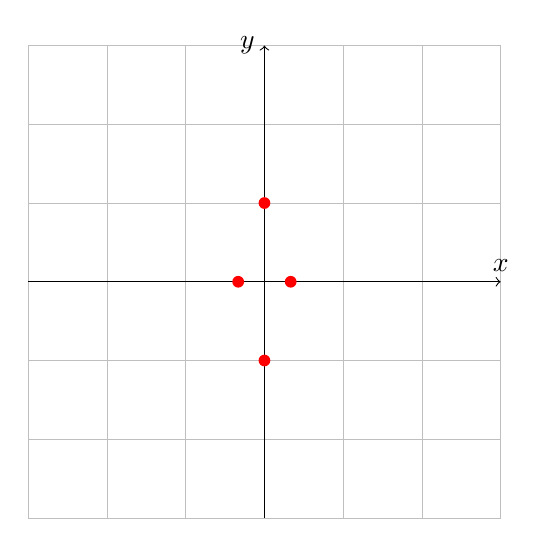
\begin{tikzpicture}
          \draw[very thin,lightgray] (-3,-3) grid (3,3);
          \draw[->] (-3,0)--(3,0) node[above]{$x$};
          \draw[->] (0,-3)--(0,3) node[left]{$y$};
          \node[fill=red,inner sep=1.5pt,shape=circle] (I1) at (-1/3,0) {} ;
          \node[fill=red,inner sep=1.5pt,shape=circle] (I2) at (1/3,0) {} ;
          \node[fill=red,inner sep=1.5pt,shape=circle] (I3) at (0,-1) {} ;
          \node[fill=red,inner sep=1.5pt,shape=circle] (I4) at (0,1) {} ;
        \end{tikzpicture}
        &
        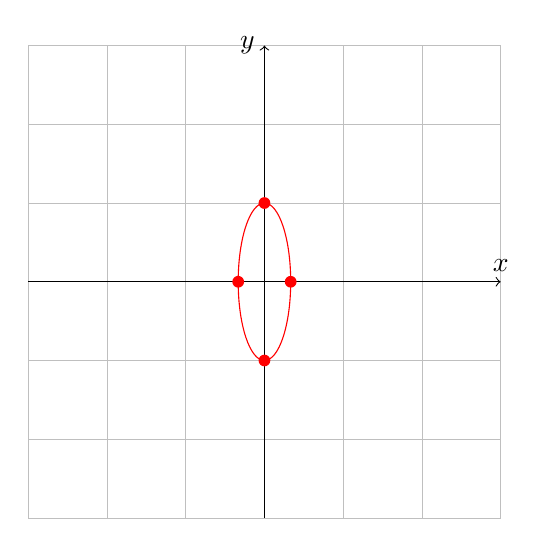
\begin{tikzpicture}
          \draw[very thin,lightgray] (-3,-3) grid (3,3);
          \draw[->] (-3,0)--(3,0) node[above]{$x$};
          \draw[->] (0,-3)--(0,3) node[left]{$y$};
          \node[fill=red,inner sep=1.5pt,shape=circle] (I1) at (-1/3,0) {} ;
          \node[fill=red,inner sep=1.5pt,shape=circle] (I2) at (1/3,0) {} ;
          \node[fill=red,inner sep=1.5pt,shape=circle] (I3) at (0,-1) {} ;
          \node[fill=red,inner sep=1.5pt,shape=circle] (I4) at (0,1){} ;
          \draw[red] (0,0) ellipse (1/3 and 1);
        \end{tikzpicture}
        \\
        \mbox{(a) intercepts}
        &
        \mbox{(b) completed}
        \end{array}$
      \caption{Graphing $9x^2+y^2 = 1$}
      \label{fig:9x2+y2=1}
    \end{figure}
  \item %$\ds x=y^2+4$
    Rearranging,
    \begin{equation*}
      x=y^2+4 \implies x-4 = y^2
    \end{equation*}
    which is the equation of a parabola with vertex $(4,0)$ opening to
    the right.  Picking $y=1$ gives $(5,1)$ as another point on the
    parabola.
    See Figure~\ref{fig:x=y2+4}.
    \begin{figure}[htbp]
      \centering
      $\begin{array}{c@{\hspace{1cm}}c}
        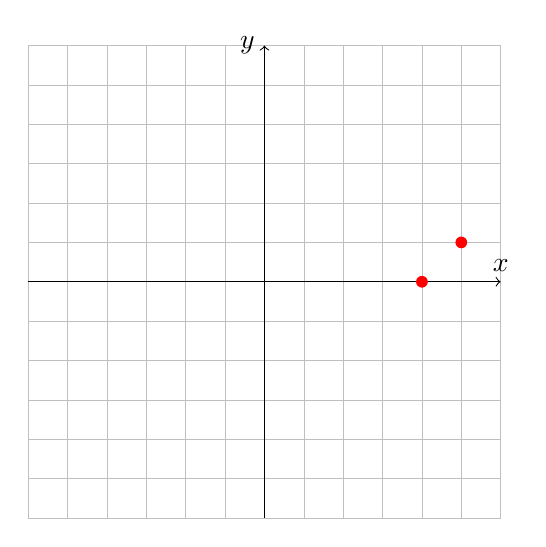
\begin{tikzpicture}[scale=0.5]
          \draw[very thin,lightgray] (-6,-6) grid (6,6);
          \draw[->] (-6,0)--(6,0) node[above]{$x$};
          \draw[->] (0,-6)--(0,6) node[left]{$y$};
          \node[fill=red,inner sep=1.5pt,shape=circle] (V) at (4,0) {} ;
          \node[fill=red,inner sep=1.5pt,shape=circle] (P) at (5,1) {} ;
        \end{tikzpicture}
        &
        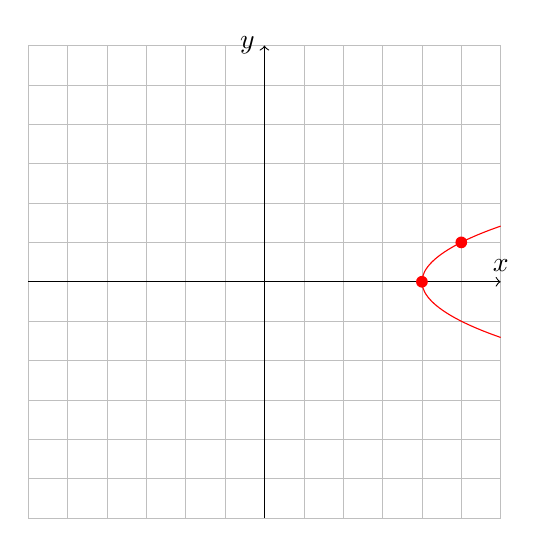
\begin{tikzpicture}[scale=0.5]
          \draw[very thin,lightgray] (-6,-6) grid (6,6);
          \draw[->] (-6,0)--(6,0) node[above]{$x$};
          \draw[->] (0,-6)--(0,6) node[left]{$y$};
          \node[fill=red,inner sep=1.5pt,shape=circle] (V) at (4,0) {} ;
          \node[fill=red,inner sep=1.5pt,shape=circle] (P) at (5,1) {}
          ;
          \draw[red,rotate=-90] (0,4) parabola ({sqrt(2)},6);
          \draw[red,rotate=-90] (0,4) parabola ({-sqrt(2)},6);
        \end{tikzpicture}
        \\
        \mbox{(a) vertex, point}
        &
        \mbox{(b) completed}
        \end{array}$
      \caption{Graphing $x=y^2+4$}
      \label{fig:x=y2+4}
    \end{figure}
  \item %$\ds 16y^2-9x^2=25$
    Dividing through by $25$,
    \begin{equation*}
      -\frac{9x^2}{25} + \frac{16y^2}{25} = 1
      \implies
      -\frac{x^2}{(5/3)^2} + \frac{y^2}{(5/4)^2} = 1
    \end{equation*}
    This is the equation of a hyperbola opening upward and downward,
    with $y$-intercepts $(-5/4,0)$ and $(5/4,0)$ and asymptotes 
    \begin{equation*}
      \frac{x}{5/3} + \frac{y}{5/4} = 0, 
      \qquad 
      -\frac{x}{5/3} + \frac{y}{5/4} = 0
    \end{equation*}
    See Figure~\ref{fig:16y2-9x2=25}.
    \begin{figure}[htbp]
      \centering
      $\begin{array}{c@{\hspace{1cm}}c}
        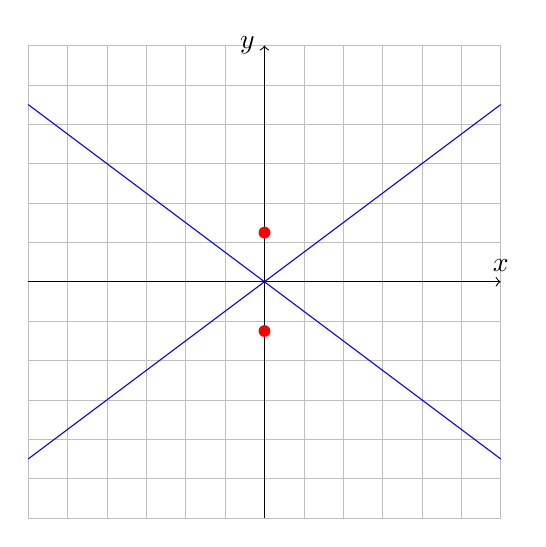
\begin{tikzpicture}[scale=0.5]
          \draw[very thin,lightgray] (-6,-6) grid (6,6);
          \draw[->] (-6,0)--(6,0) node[above]{$x$};
          \draw[->] (0,-6)--(0,6) node[left]{$y$};
          \node[fill=red,inner sep=1.5pt,shape=circle] (I1) at (0,-5/4) {} ;
          \node[fill=red,inner sep=1.5pt,shape=circle] (I2) at (0,5/4) {};
          \draw[blue] (-6,4.5)--(6,-4.5);
          \draw[blue] (-6,-4.5)--(6,4.5);
        \end{tikzpicture}
        &
        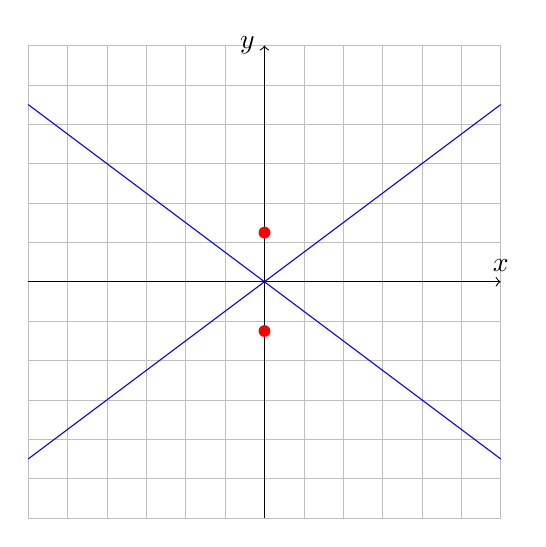
\begin{tikzpicture}[scale=0.5]
          \draw[very thin,lightgray] (-6,-6) grid (6,6);
          \draw[->] (-6,0)--(6,0) node[above]{$x$};
          \draw[->] (0,-6)--(0,6) node[left]{$y$};
          \node[fill=red,inner sep=1.5pt,shape=circle] (I1) at (0,-5/4) {} ;
          \node[fill=red,inner sep=1.5pt,shape=circle] (I2) at (0,5/4) {};
          \draw[blue] (-6,4.5)--(6,-4.5);
          \draw[blue] (-6,-4.5)--(6,4.5);
          \clip (-6,-6)--(6,-6)--(6,6)--(-6,6)--cycle;
          \draw[red,domain=-6:6] plot[id=hyp1] function{sqrt((25+9*x*x)/16)};
          \draw[red,domain=-6:6] plot[id=hyp2] function{-sqrt((25+9*x*x)/16)};
        \end{tikzpicture}
        \\
        \mbox{(a) vertices, asymptotes}
        &
        \mbox{(b) completed}
        \end{array}$
      \caption{Graphing $16y^2-9x^2=25$}
      \label{fig:16y2-9x2=25}
    \end{figure}
  \item %$\ds y^2-x^2+4y=10$ % EJD: should make 10 -> 12
    Completing the square,
    \begin{equation*}
      -x^2 + y^2 + 4y + 4 = 14
      \implies -x^2 + (y+2)^2 = 14
      \implies -\frac{x^2}{(\sqrt{14})^2} +
      \frac{(y+2)^2}{(\sqrt{14})^2} = 1
    \end{equation*}
    We begin by graphing the hyperbola
    \begin{equation*}
      -\frac{x^2}{(\sqrt{14})^2} + \frac{y^2}{(\sqrt{14})^2} = 1
    \end{equation*}
    which opens upward and downward, has $y$-intercepts
    $(0,-\sqrt{14})$ and $(0,\sqrt{14})$, and has asymptotes
    \begin{equation*}
      \frac{x}{\sqrt{14}}+\frac{y}{\sqrt{14}} = 0,
      \qquad
      -\frac{x}{\sqrt{14}}+\frac{y}{\sqrt{14}} = 0
    \end{equation*}
    in other words $x+y=0$ and $-x+y=0$.  See Figure~\ref{fig:y2-x2+4y=10}(a).
    Finally, we shift the diagram so that the center moves from
    $(0,0)$ to $(0,-2)$ to get the answer to the question.  See
    Figure~\ref{fig:y2-x2+4y=10}(b). 
    \begin{figure}[htbp]
      \centering
      $\begin{array}{c@{\hspace{1cm}}c}
        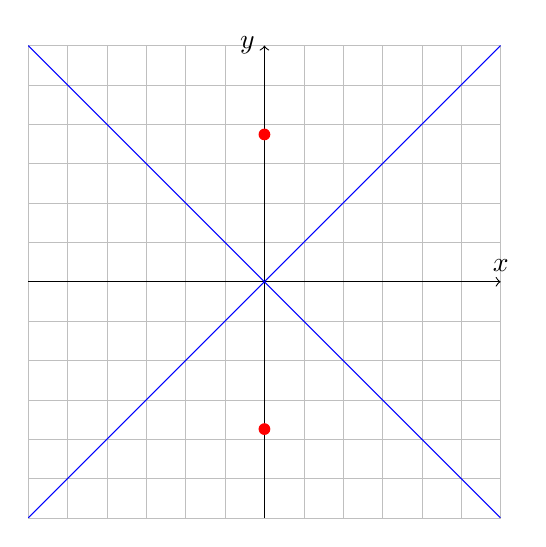
\begin{tikzpicture}[scale=0.5]
          \draw[very thin,lightgray] (-6,-6) grid (6,6);
          \draw[->] (-6,0)--(6,0) node[above]{$x$};
          \draw[->] (0,-6)--(0,6) node[left]{$y$};
          \clip (-6,-6)--(6,-6)--(6,6)--(-6,6)--cycle;
          \node[fill=red,inner sep=1.5pt,shape=circle] (I1) at (0,{-sqrt(14)}) {} ;
          \node[fill=red,inner sep=1.5pt,shape=circle] (I2) at (0,{sqrt(14)}) {};
          \draw[blue] (-6,6)--(6,-6);
          \draw[blue] (-6,-6)--(6,6);
          \draw[red,domain=-6:6] plot[id=hyp3] function{sqrt(14+x*x)};
          \draw[red,domain=-6:6] plot[id=hyp4]
          function{-sqrt(14+x*x)};
        \end{tikzpicture}
        &
        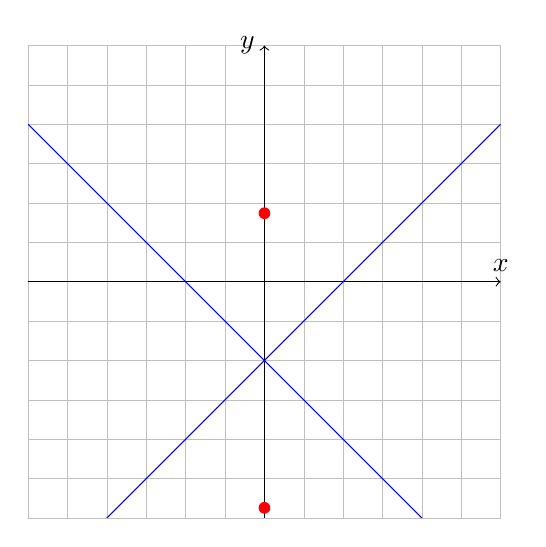
\begin{tikzpicture}[scale=0.5]
          \draw[very thin,lightgray] (-6,-6) grid (6,6);
          \draw[->] (-6,0)--(6,0) node[above]{$x$};
          \draw[->] (0,-6)--(0,6) node[left]{$y$};
          \clip (-6,-6)--(6,-6)--(6,6)--(-6,6)--cycle;
          \node[fill=red,inner sep=1.5pt,shape=circle] (I1) at (0,{-sqrt(14)-2}) {} ;
          \node[fill=red,inner sep=1.5pt,shape=circle] (I2) at (0,{sqrt(14)-2}) {};
          \draw[blue] (-6,6-2)--(6,-6-2);
          \draw[blue] (-6,-6-2)--(6,6-2);
          \draw[red,domain=-6:6] plot[id=hyp5] function{(sqrt(14+x*x)-2)};
          \draw[red,domain=-6:6] plot[id=hyp6] function{(-sqrt(14+x*x)-2)};
        \end{tikzpicture}
        \\
        \mbox{(a) Graph of $-x^2+y^2=14$}
        &
        \mbox{(b) completed}
        \end{array}$
      \caption{Graphing $y^2-x^2+4y=10$}
      \label{fig:y2-x2+4y=10}
    \end{figure}
  \end{enumerate}
\item %(Based on C.33--34) Sketch the region bounded by the curves.
  \begin{enumerate}
  \item %$\ds y=-x^2$, $y=5x$
    A quick sketch (with a large-enough scale on the $y$-axis) shows
    that there seem to be two intersection points.  See
    Figure~\ref{fig:y=-x2ANDy=5x}(a).  To find the coordinates of the
    intersection points, solve
    \begin{equation*}
      -x^2 = y = 5x \implies -x^2=5x \implies x^2+5x=0 \implies
      (x+5)x=0
    \end{equation*}
    with roots $x=-5$, $x=0$ and corresponding $y$-values
    $y=5(-5)=-25$ and $y=5(0)=0$.  So the intersection points are
    $(-5,-25)$ and $(0,0)$.  See Figure~\ref{fig:y=-x2ANDy=5x}(b).
    \begin{figure}[htbp]
      \centering
      $\begin{array}{c@{\hspace{1cm}}c}
        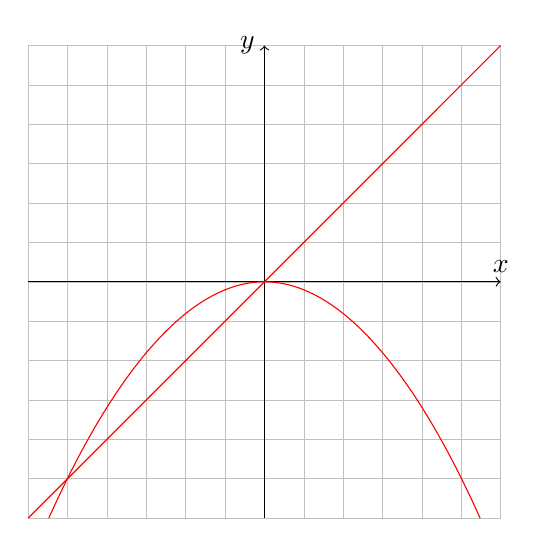
\begin{tikzpicture}[xscale=0.5,yscale=0.1]
          \draw[ystep=5,very thin,lightgray] (-6,-30) grid (6,30);
          \draw[->] (-6,0) -- (6,0) node[above]{$x$};
          \draw[->] (0,-30)--(0,30) node[left]{$y$};
          \draw[red] (0,0) parabola ({-sqrt(30)},-30);
          \draw[red] (0,0) parabola ({sqrt(30)},-30);
          \draw[red] (-6,-30)--(6,30);
        \end{tikzpicture}
        &
        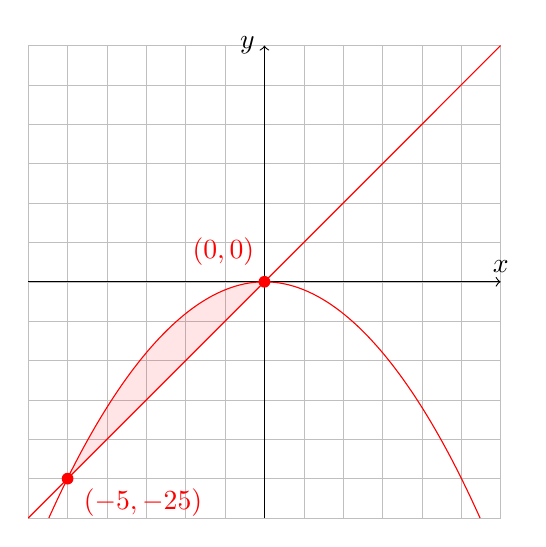
\begin{tikzpicture}[xscale=0.5,yscale=0.1]
          \draw[ystep=5,very thin,lightgray] (-6,-30) grid (6,30);
          \draw[->] (-6,0) -- (6,0) node[above]{$x$};
          \draw[->] (0,-30)--(0,30) node[left]{$y$};
          \clip (-6,-30)--(6,-30)--(6,30)--(-6,30)--cycle;
          \draw[red] (0,0) parabola ({-sqrt(30)},-30);
          \draw[red] (0,0) parabola ({sqrt(30)},-30);
          \draw[red] (-6,-30)--(6,30);
          \draw node[fill=red,inner %
            sep=1.5pt,shape=circle,label={[red]95:$(0,0)$}] (I0) at %
          (0,0) {}; 
          \draw node[fill=red,inner %
            sep=1.5pt,shape=circle,label={[red]355:$(-5,-25)$}] (I1) %
          at (-5,-25) {};
          \fill[red,very nearly transparent] (0,0) parabola (-5,-25)
          -- cycle;
        \end{tikzpicture}
        \\
        \mbox{(a) Sketch of curves}
        &
        \mbox{(b) Intersection points and region}
      \end{array}$
      \caption{Graphing region between $y=-x^2$ and $y=5x$}
      \label{fig:y=-x2ANDy=5x}
    \end{figure}
  \item %$\ds y=x^2-1$, $y=2x+2$
    A quick sketch of the curves again indicates that there should be
    two intersection points.  See Figure~\ref{fig:y=x2-1ANDy=2x+2}(a).
    To find the intersection points, solve
    \begin{equation*}
      x^2-1 = y = 2x+2 \implies x^2-1 = 2x+2 \implies x^2-2x-3 = 0
      \implies (x+1)(x-3)=0
    \end{equation*}
    so the intersection points are $(-1,0)$ and $(3,8)$.  See
    Figure~\ref{fig:y=x2-1ANDy=2x+2}(b). 
    \begin{figure}[htbp]
      \centering
      $\begin{array}{c@{\hspace{1cm}}c}
        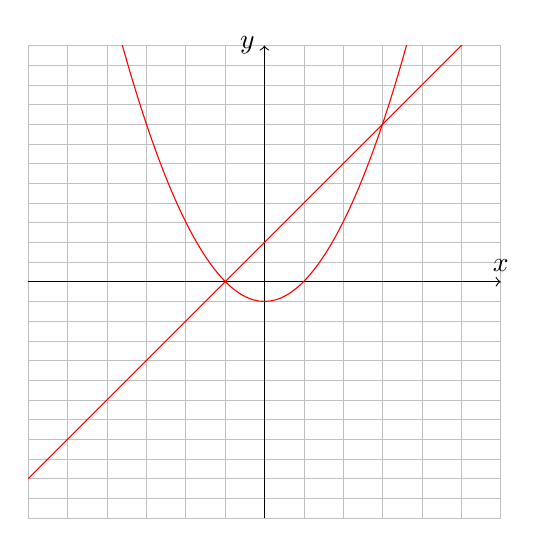
\begin{tikzpicture}[xscale=0.5,yscale=0.25]
          \draw[very thin,lightgray] (-6,-12) grid (6,12);
          \draw[->] (-6,0) -- (6,0) node[above]{$x$};
          \draw[->] (0,-12) -- (0,12) node[left]{$y$};
          \clip (-6,-12)--(6,-12)--(6,12)--(-6,12)--cycle;
          \draw[red] (0,-1) parabola (-6,35);
          \draw[red] (0,-1) parabola (6,35);
          \draw[red] (-6,-10)--(6,14);
        \end{tikzpicture}
        &
        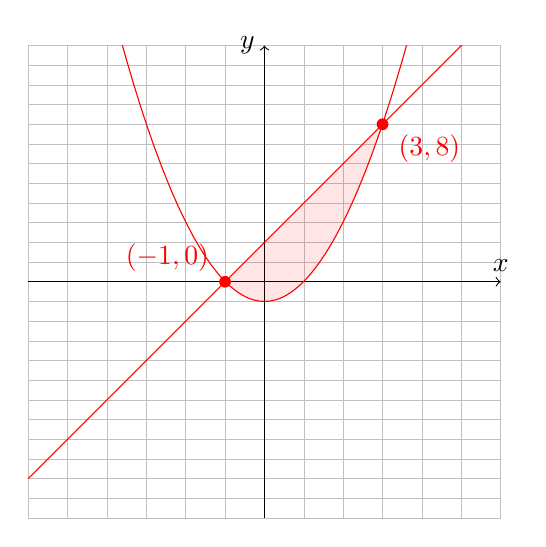
\begin{tikzpicture}[xscale=0.5,yscale=0.25]
          \draw[very thin,lightgray] (-6,-12) grid (6,12);
          \draw[->] (-6,0) -- (6,0) node[above]{$x$};
          \draw[->] (0,-12) -- (0,12) node[left]{$y$};
          \clip (-6,-12)--(6,-12)--(6,12)--(-6,12)--cycle;
          \draw[red] (0,-1) parabola (-6,35);
          \draw[red] (0,-1) parabola (6,35);
          \draw[red] (-6,-10)--(6,14);
          \draw node[fill=red,inner %
            sep=1.5pt,shape=circle,label={[red]175:$(-1,0)$}] (I0) at %
          (-1,0) {}; 
          \draw node[fill=red,inner %
            sep=1.5pt,shape=circle,label={[red]355:$(3,8)$}] (I1) %
          at (3,8) {};
          \fill[red,very nearly transparent] (-1,0) parabola[bend at
            end] (0,-1) parabola (3,8) -- cycle;
        \end{tikzpicture}
        \\
        \mbox{(a) Sketch of curves}
        &
        \mbox{(b) Intersection points and region}
      \end{array}$
      \caption{Graphing the region between $y=x^2-1$ and $y=2x+2$}
      \label{fig:y=x2-1ANDy=2x+2}
    \end{figure}
  \end{enumerate}
\item %(Based on C.31--32) Identify the type of curve and sketch the graph.
  %Do not plot points.  Just use the standard graphs given in the textbook
  %and shift if necessary.
  \begin{enumerate}
  \item %$\ds x^2+4y^2-32y=16$ % EJD: make it =17?
    Completing the square,
    \begin{equation*}
      x^2 + 4(y^2-8y+16-16) = 16 \implies x^2 + 4(y-4)^2 = 80
    \end{equation*}
    Putting the equation in standard form,
    \begin{equation*}
      \frac{x^2}{(\sqrt{80})^2} + \frac{(y-4)^2}{(\sqrt{20})} = 1
    \end{equation*}
    The figure is an ellipse.  We first graph $x^2/(\sqrt{80})^2+
    y^2/(\sqrt{20})^2 = 1$ by locating the vertices, namely
    $(-\sqrt{80},0)$, $(\sqrt{80},0)$, $(0,-\sqrt{20})$,
    $(0,\sqrt{20})$ and joining them by appropriate arcs.  See
    Figure~\ref{fig:x2+4y2-32y=16}(a). 
    Then we shift the resulting figure so the center moves from
    $(0,0)$ to $(0,4)$.  See Figure~\ref{fig:x2+4y2-32y=16}(b).
    \begin{figure}[htbp]
      \centering
      $\begin{array}{c@{\hspace{1cm}}c}
        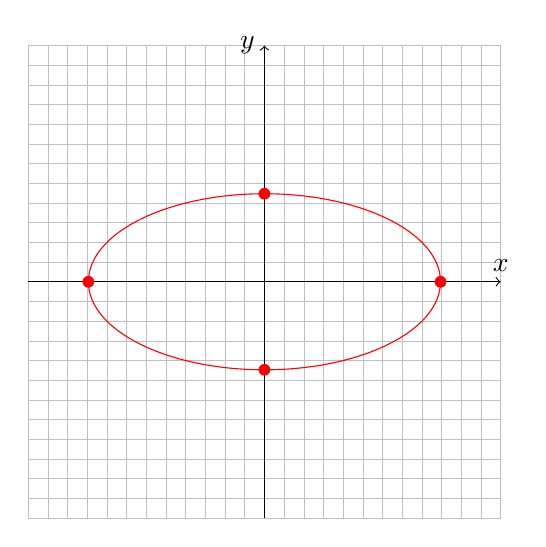
\begin{tikzpicture}[scale=0.25]
          \draw[very thin,lightgray] (-12,-12) grid (12,12);
          \draw[->] (-12,0) -- (12,0) node[above]{$x$};
          \draw[->] (0,-12) -- (0,12) node[left]{$y$};
          \clip (-12,-12)--(12,-12)--(12,12)--(-12,12)--cycle;
          \draw node[fill=red,inner %
            sep=1.5pt,shape=circle] (I0) at %
          ({-sqrt(80)},0) {}; 
          \draw node[fill=red,inner %
            sep=1.5pt,shape=circle] (I1) %
          at ({sqrt(80)},0) {};
          \draw node[fill=red,inner %
            sep=1.5pt,shape=circle] (I2) at %
          (0,{-sqrt(20)}) {}; 
          \draw node[fill=red,inner %
            sep=1.5pt,shape=circle] (I3) %
          at (0,{sqrt(20)}) {};
          \draw[red] (0,0) ellipse ({sqrt(80)} and {sqrt(20)});
        \end{tikzpicture}
        &
        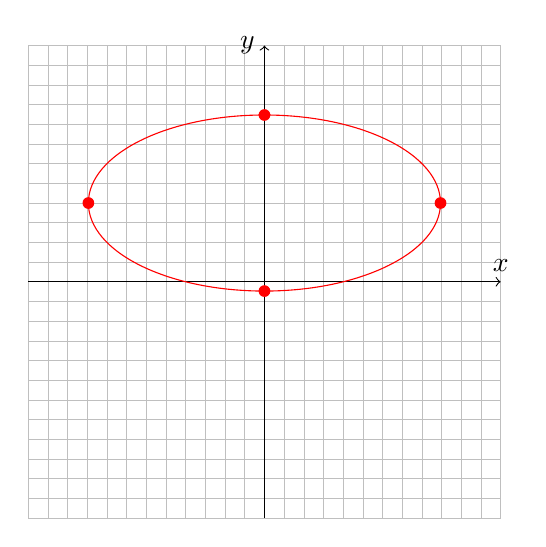
\begin{tikzpicture}[scale=0.25]
          \draw[very thin,lightgray] (-12,-12) grid (12,12);
          \draw[->] (-12,0) -- (12,0) node[above]{$x$};
          \draw[->] (0,-12) -- (0,12) node[left]{$y$};
          \clip (-12,-12)--(12,-12)--(12,12)--(-12,12)--cycle;
          \draw node[fill=red,inner %
            sep=1.5pt,shape=circle] (I0) at %
          ({-sqrt(80)},4) {}; 
          \draw node[fill=red,inner %
            sep=1.5pt,shape=circle] (I1) %
          at ({sqrt(80)},4) {};
          \draw node[fill=red,inner %
            sep=1.5pt,shape=circle] (I2) at %
          (0,{-sqrt(20)+4}) {}; 
          \draw node[fill=red,inner %
            sep=1.5pt,shape=circle] (I3) %
          at (0,{sqrt(20)+4}) {};
          \draw[red] (0,4) ellipse ({sqrt(80)} and {sqrt(20)});
        \end{tikzpicture}
        \\
        \mbox{(a) Graph of $x^2/80+y^2/20=1$}
        &
        \mbox{(b) Center shifted to $(0,4)$}
      \end{array}$
      \caption{Graphing $x^2+4y^2-32y=16$}
      \label{fig:x2+4y2-32y=16}
    \end{figure}
  \item %$\ds 9x^2-4y^2-6x+5=0$ % EJD: we haven't yet graphed
        %hyperbola opening left and right!!
    Completing the square,
    \begin{equation*}
      9\left(x^2-\frac{2}{3}x+\frac{1}{9}-\frac{1}{9}\right) - 4y^2 =
      -5
      \implies 9\left(x-\frac{1}{3}\right) - 4y^2 = -4
    \end{equation*}
    Putting the equation into standard form,
    \begin{equation*}
      -\frac{(x-1/3)^2}{(2/3)^2} + \frac{y^2}{1^2} = 1
    \end{equation*}
    We first graph $-x^2/(2/3)^2 + y^2/1^2 = 1$.  It is
    a hyperbola opening upwards and downwards, with $y$-intercepts
    $(0,-1)$ and $(0,1)$ and asymptotes
    \begin{equation*}
      \frac{x}{2/3} + \frac{y}{1} = 0, \qquad
      -\frac{x}{2/3} + \frac{y}{1} = 0
    \end{equation*}
    See Figure~\ref{fig:9x2-4y2-6x+5=0}(a).  Then we shift the graph
    so that the center moves from $(0,0)$ to $(1/3,0)$.  See
    Figure~\ref{fig:9x2-4y2-6x+5=0}(b). 
    \begin{figure}[htbp]
      \centering
      $\begin{array}{c@{\hspace{1cm}}c}
        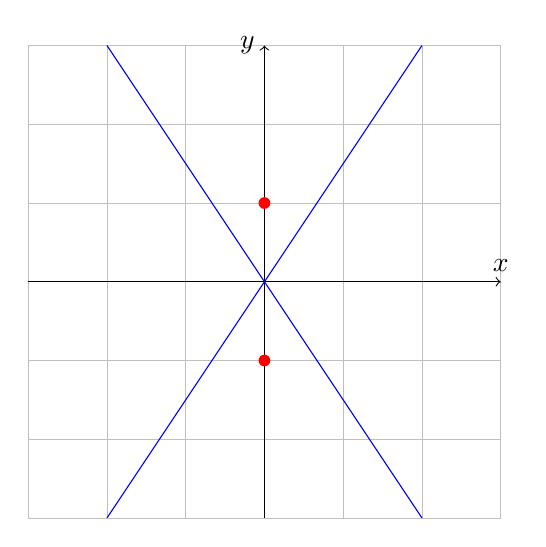
\begin{tikzpicture}[scale=1.0]
          \draw[very thin,lightgray] (-3,-3) grid (3,3);
          \draw[->] (-3,0) -- (3,0) node[above]{$x$};
          \draw[->] (0,-3) -- (0,3) node[left]{$y$};
          \clip (-3,-3)--(3,-3)--(3,3)--(-3,3)--cycle;
          \draw node[fill=red,inner %
            sep=1.5pt,shape=circle] (I0) at %
          (0,-1) {}; 
          \draw node[fill=red,inner %
            sep=1.5pt,shape=circle] (I1) %
          at (0,1) {};
          \draw[blue] (-2,3)--(2,-3);
          \draw[blue] (-2,-3)--(2,3);
          \draw[red,domain=-3:3] plot[id=hyp07] function{sqrt(1+9*x*x/4)};
          \draw[red,domain=-3:3] plot[id=hyp08] function{-sqrt(1+9*x*x/4)};
        \end{tikzpicture}
        &
        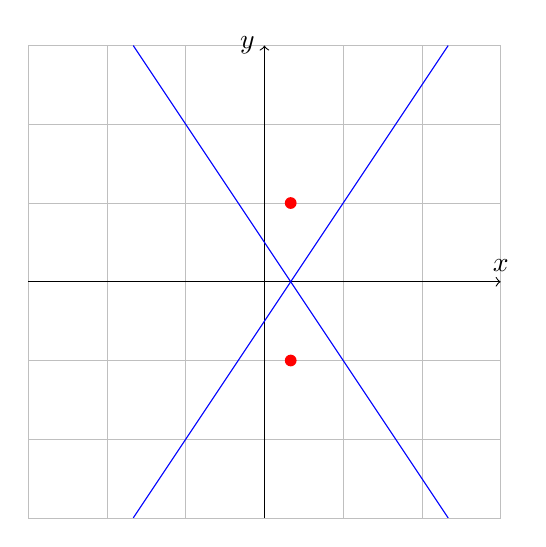
\begin{tikzpicture}[scale=1.0]
          \draw[very thin,lightgray] (-3,-3) grid (3,3);
          \draw[->] (-3,0) -- (3,0) node[above]{$x$};
          \draw[->] (0,-3) -- (0,3) node[left]{$y$};
          \clip (-3,-3)--(3,-3)--(3,3)--(-3,3)--cycle;
          \draw node[fill=red,inner %
            sep=1.5pt,shape=circle] (I0) at %
          (0.33333,-1) {}; 
          \draw node[fill=red,inner %
            sep=1.5pt,shape=circle] (I1) %
          at (0.33333,1) {};
          \draw[blue] (-2+0.33333,3)--(2+0.33333,-3);
          \draw[blue] (-2+0.33333,-3)--(2+0.33333,3);
          \draw[red,domain=-3:3] plot[id=hyp09]
          function{sqrt(1+9*(x-0.33333)**2/4)};
          \draw[red,domain=-3:3] plot[id=hyp10] function{-sqrt(1+9*(x-0.33333)**2/4)};
        \end{tikzpicture}
        \\
        \mbox{(a) Graph of $-x^2/(2/3)^2+y^2/1^2=1$}
        &
        \mbox{(b) Center shifted to $(1/3,0)$}
      \end{array}$
      \caption{Graphing $9x^2-4y^2-6x+5=0$}
      \label{fig:9x2-4y2-6x+5=0}
    \end{figure}
  \end{enumerate}
\item %(Based on C.35) Find an equation of the parabola with vertex $(1,5)$
  %that opens downward and passes through the point $(-1,-4)$.
  A parabola in standard position which opens downward has equation
  \begin{equation*}
    y=-ax^2
  \end{equation*}
  Shifting the vertex from $(0,0)$ to $(1,5)$, the equation becomes 
  \begin{equation*}
    y-5 = -a(x-1)^2
  \end{equation*}
  Since the parabola passes through $(-1,-4)$, the values
  $(x,y)=(-1,-4)$ must satisfy the equation so we have
  \begin{equation*}
    -4-5 = -a(-1-1)^2 \implies -9 = -a (2)^2 \implies a = \frac{9}{4}
  \end{equation*}
  So the parabola has equation
  \begin{equation*}
    y-5 = -\frac{9}{4} (x-1)^2
  \end{equation*}
  You might want to check the correctness of that equation by graphing
  it. 
\item %(Based on C.37--40) Sketch the graph of the set.
  \begin{enumerate}
  \item %$\ds \{(x,y)|x^2+y^2\le 4\}$
    The solution set is the set of all points the distance from the
    origin of which is less than $\sqrt{4}$, in other words the inside
    of a circle of center $(0,0)$ and radius $2$.  See
    Figure~\ref{fig:graph-ineq1}(a). 
    \begin{figure}[htbp]
      \centering
      $\begin{array}{c@{\hspace{1cm}}c}
        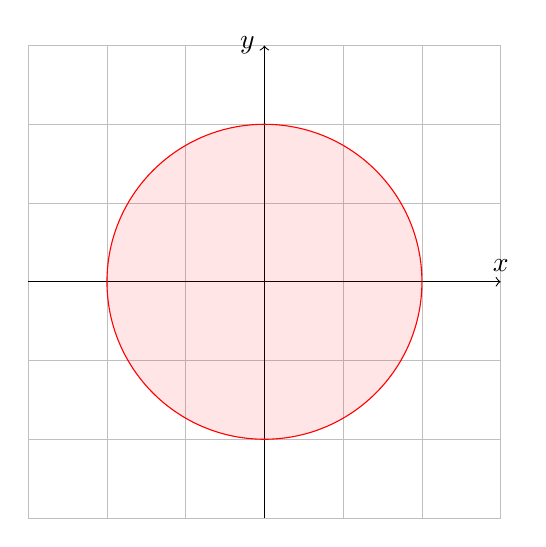
\begin{tikzpicture}[scale=1.0]
          \draw[very thin,lightgray] (-3,-3) grid (3,3);
          \draw[->] (-3,0) -- (3,0) node[above]{$x$};
          \draw[->] (0,-3) -- (0,3) node[left]{$y$};
          \clip (-3,-3)--(3,-3)--(3,3)--(-3,3)--cycle;
          \fill[red,very nearly transparent] (0,0) circle (2);
          \draw[red] (0,0) circle (2);
        \end{tikzpicture}
        &
        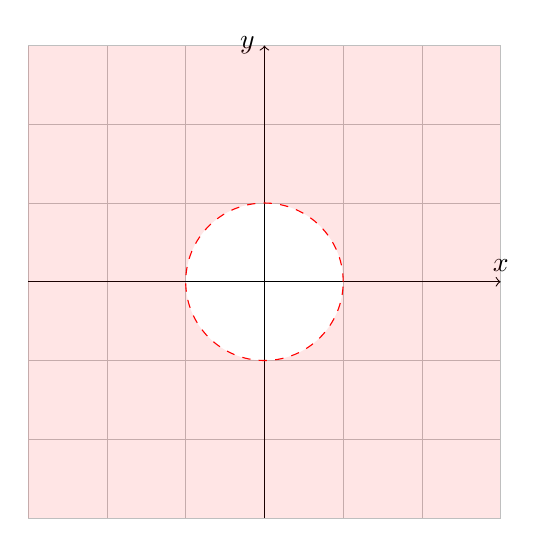
\begin{tikzpicture}[scale=1.0]
          \draw[very thin,lightgray] (-3,-3) grid (3,3);
          \draw[->] (-3,0) -- (3,0) node[above]{$x$};
          \draw[->] (0,-3) -- (0,3) node[left]{$y$};
          %\clip (-3,-3)--(3,-3)--(3,3)--(-3,3)--cycle;
          \begin{scope}[even odd rule]
            \clip {(-3,-3)--(3,-3)--(3,3)--(-3,3)--cycle (0,0) circle (1)};
            \fill[red,very nearly transparent] (-3,-3)--(3,-3)--(3,3)--(-3,3)--cycle;
          \end{scope}
          \draw[red,dashed] (0,0) circle (1);
        \end{tikzpicture}
        \\
        \mbox{(a) Graph of $x^2+y^2\le 4$}
        &
        \mbox{(b) Graph of $x^2+y^2>1$}
      \end{array}$
      \caption{Graphing some inequalities} % EJD: refer to problem number
      \label{fig:graph-ineq1}
    \end{figure}
  \item %$\ds \{(x,y)|x^2+y^2>1\}$
    This question is similar to the previous, however the set of
    points is the set that is not inside or on the unit circle.  See
    Figure~\ref{fig:graph-ineq1}(b). 
  \item %$\ds \{(x,y)|y>x^2-2x\}$
    Completing the square we have
    \begin{equation*}
      y+1 > (x-1)^2
    \end{equation*}
    The region is the set of all points above a parabola with vertex
    $(1,-1)$ opening upwards.
    \begin{figure}[htbp]
      \centering
      $\begin{array}{c@{\hspace{1cm}}c}
        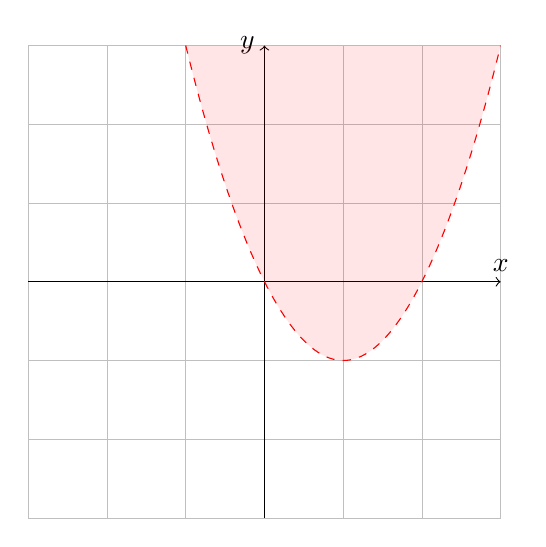
\begin{tikzpicture}[scale=1.0]
          \draw[very thin,lightgray] (-3,-3) grid (3,3);
          \draw[->] (-3,0) -- (3,0) node[above]{$x$};
          \draw[->] (0,-3) -- (0,3) node[left]{$y$};
          \clip (-3,-3)--(3,-3)--(3,3)--(-3,3)--cycle;
          \fill[red,very nearly transparent] (-1,3) parabola[bend at end]
            (1,-1) parabola (3,3) -- cycle;
          \draw[red,dashed] (-1,3) parabola[bend at end] (1,-1) parabola (3,3);
        \end{tikzpicture}
        &
        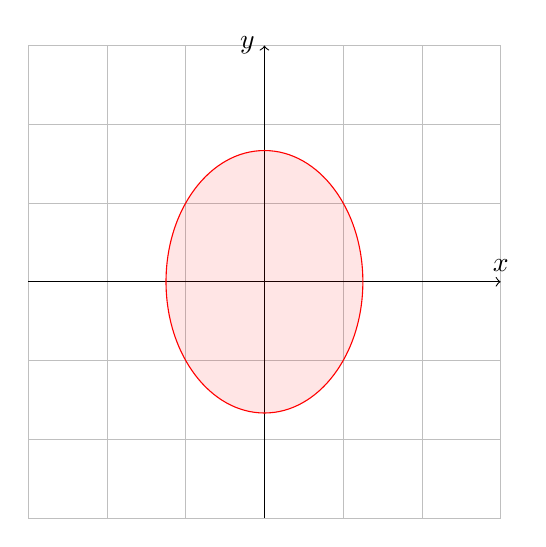
\begin{tikzpicture}[scale=1.0]
          \draw[very thin,lightgray] (-3,-3) grid (3,3);
          \draw[->] (-3,0) -- (3,0) node[above]{$x$};
          \draw[->] (0,-3) -- (0,3) node[left]{$y$};
          \fill[red,very nearly transparent] (0,0) ellipse (5/4 and 5/3);
          \draw[red] (0,0) ellipse (5/4 and 5/3);
        \end{tikzpicture}
        \\
        \mbox{(a) Graph of $y>x^2-2x$}
        &
        \mbox{(b) Graph of $16x^2+9y^2\le 25$}
      \end{array}$
      \caption{Graphing some other inequalities} % EJD: refer to problem number
      \label{fig:graph-ineq2}
    \end{figure}
  \item %$\ds \{(x,y)|16x^2+9y^2\le 25\}$
    In standard form, the equation is 
    \begin{equation*}
      \frac{x^2}{(5/4)^2} + \frac{y^2}{(5/3)^2} \le 1
    \end{equation*}
    so the boundary of the region is an ellipse in standard position
    with vertices $(-5/4,0)$, $(5/4,0)$, $(0,-5/3)$, $(0,5/3)$.  Since
    the ellipse is a flattened circle, and the $\le 1$ condition means
    everything inside and on the circle in the circle case, we graph
    all points inside and on the ellipse.
  \end{enumerate}
\item %(Based on C.10) Under what condition on the coefficients $a$, $b$, and
  %$c$ does the equation $x^2+4y^2+ax+by+c=0$ represent an ellipse?  When
  %that condition is satisfied, find the center of the ellipse.
  Completing the square,
  \begin{equation*}
    x^2+ax + \frac{a^2}{4} - \frac{a^2}{4} + 
    4\left(y^2 + \frac{b}{4} y + \frac{b^2}{64} -
    \frac{b^2}{64}\right)
    = -c
  \end{equation*}
  Simplifying,
  \begin{equation*}
    \left(x+\frac{a}{2}\right)^2 + 4\left(y+\frac{b}{8}\right)^2 = 
    \frac{a^2}{4} - \frac{b^2}{16} - c
  \end{equation*}
  Since the LHS is a sum of squares, it must always be $\ge 0$.  So
  for the equation to represent an ellipse, we must have the RHS $\ge
  0$ (what happens if the RHS $=0$?).  So the condition for the
  equation to represent an ellipse is
  \begin{equation*}
    \frac{a^2}{4} - \frac{b^2}{16} - c > 0
  \end{equation*}
  When that condition is satisfied, the center of the ellipse is 
  \begin{equation*}
    \left(-\frac{a}{2},-\frac{b}{8}\right)
  \end{equation*}
\end{enumerate}
\end{document}

